\chapter{Текстовые задачи и финансовые модели}\label{chap:exam-models}\markright{Глава 17}
\section{От условия к уравнению}
\begin{definition}\term{Математическая модель} (\emph{mathematical model}) --- описание существенных величин, связей и ограничений задачи математическими средствами. Полученное решение интерпретируют в исходных единицах и проверяют по условию.\end{definition}
Удобный порядок: выбрать неизвестные с единицами; указать допустимые значения; составить таблицу величин; выразить отношения; решить уравнение или систему; проверить ответ. Положительная масса, целое количество предметов и время не раньше начала процесса --- части модели, а не необязательные замечания после вычислений.
\section{Движение и средняя скорость}
При постоянной скорости \(s=vt\). Для нескольких участков пути полное время складывается, поэтому \(v_{\rm ср}=\frac{s_1+\cdots+s_k}{t_1+\cdots+t_k}\). Среднее арифметическое скоростей подходит при равных временах, но не при произвольных участках. При движении навстречу расстояние между объектами уменьшается со скоростью \(v_1+v_2\); при погоне в одном направлении --- со скоростью \(v_1-v_2>0\). На реке при собственной скорости \(v\) и скорости течения \(u\) скорости по течению и против него равны \(v+u\) и \(v-u\); движение против течения требует \(v>u\).
\begin{example}Пешеход проходит \(6\) км со скоростью \(3\) км/ч и возвращается со скоростью \(6\) км/ч. Время \(2+1=3\) часа, средняя скорость \(\frac{12}{3}=4\) км/ч. Среднее \(4{,}5\) здесь неверно: медленный участок занял больше времени.\end{example}
\begin{example}Два велосипедиста проезжают по \(60\) км, скорости отличаются на \(5\) км/ч, времена --- на один час. Для меньшей скорости \(v>0\): \(\frac{60}v-\frac{60}{v+5}=1\). Получаем \(v^2+5v-300=0\), корни \(15,-20\). Допустим только \(v=15\), вторая скорость \(20\) км/ч.\end{example}
\par\addvspace{2pt}\begin{lrbox}{\CatFlowBox}\begin{minipage}[t]{\linewidth}
\setlength{\parskip}{2pt}\setlength{\columnsep}{4.5mm}\setlength{\intextsep}{0pt}
\begin{wrapfigure}[12]{r}{54mm}

\includegraphics[width=54mm,height=58mm,keepaspectratio]{images/unique/art-206.png}
\end{wrapfigure}
В задаче о движении сначала выясни, какие события происходят одновременно и какие промежутки сравниваются. Слова «на час раньше» сравнивают времена прибытия, а слова «через час после старта» задают момент наблюдения. Остановки входят в полное время поездки, если спрашивают среднюю скорость за всю поездку. Для графика пути горизонтальный участок означает отсутствие прироста пути; для графика координаты убывание означает движение в обратную сторону. Расстояние между двумя объектами находят по разности координат с модулем, а не по сумме пройденных ими путей во всех случаях. Таблица «путь --- скорость --- время» помогает сохранить эти различия при составлении уравнения.
\par\WFclear\end{minipage}\end{lrbox}%
\ifdim\dimexpr\ht\CatFlowBox+\dp\CatFlowBox\relax<60mm\dp\CatFlowBox=\dimexpr60mm-\ht\CatFlowBox\relax\fi%
\noindent\usebox{\CatFlowBox}\par\addvspace{2pt}
\section{Работа и производительность}
\begin{definition}\term{Производительность} (\emph{work rate}) --- количество работы за единицу времени. Если за \(T\) часов выполняется одна работа, постоянная производительность равна \(\frac{1}{T}\) работы в час.\end{definition}
Независимые одновременно действующие исполнители с постоянными производительностями складывают их: \(\frac1T=\frac1{T_1}+\frac1{T_2}\). При утечке или действии в противоположную сторону соответствующий расход вычитается. Формула предполагает, что исполнители не мешают друг другу и скорость работы не меняется.
\begin{example}Две трубы наполняют бак за \(6\) и \(3\) часа, слив опустошает его за \(12\) часов. Все действуют одновременно: производительность \(\frac16+\frac13-\frac1{12}=\frac5{12}\). Пустой бак заполнится за \(\frac{12}{5}=2{,}4\) часа, то есть за \(2\) часа \(24\) минуты.\end{example}
\section{Смеси, растворы и сохранение количества}
\begin{definition}\term{Массовая доля} (\emph{mass fraction}) вещества в смеси равна \(w=\frac{m_{\rm вещ}}{m_{\rm смеси}}\). В процентах это \(100w\%\).\end{definition}
При смешивании без потерь складываются массы смеси и содержащегося вещества. Для двух растворов \(w=\frac{w_1m_1+w_2m_2}{m_1+m_2}\). Массовые и объёмные доли нельзя автоматически отождествлять; для перевода нужна плотность. При испарении чистой воды масса растворённой соли сохраняется; при отливании однородного раствора уходят и вода, и соль в прежней доле.
\begin{example}К \(300\) г \(10\%\)-го раствора добавляют \(x\) г \(40\%\)-го, чтобы получить \(25\%\)-й. Соль: \(30+0{,}4x=0{,}25(300+x)\). Отсюда \(x=300\) г. Проверка: \(150\) г соли в \(600\) г раствора.\end{example}
\par\addvspace{2pt}\begin{lrbox}{\CatFlowBox}\begin{minipage}[t]{\linewidth}
\setlength{\parskip}{2pt}\setlength{\columnsep}{4.5mm}\setlength{\intextsep}{0pt}
\begin{wrapfigure}[12]{l}{54mm}

\includegraphics[width=54mm,height=58mm,keepaspectratio]{images/unique/art-207.png}
\end{wrapfigure}
Текст о смеси полезно перечитать отдельно для каждого вещества. Доля относится ко всей массе раствора, поэтому изменение знаменателя так же важно, как изменение количества соли. Если добавляется чистая вода, масса соли остаётся прежней, но общая масса растёт. Если часть однородного раствора отливают, его концентрация в этот момент не меняется, зато уменьшаются обе массы. При нескольких последовательных операциях нужно учитывать их порядок: отливание до добавления воды и после него удаляет разное количество соли. Промежуточная таблица масс делает каждое действие проверяемым. Итоговая доля при смешивании двух растворов без дополнительных процессов лежит между исходными долями.
\par\WFclear\end{minipage}\end{lrbox}%
\ifdim\dimexpr\ht\CatFlowBox+\dp\CatFlowBox\relax<59mm\dp\CatFlowBox=\dimexpr59mm-\ht\CatFlowBox\relax\fi%
\noindent\usebox{\CatFlowBox}\par\addvspace{2pt}
\section{Проценты во времени}
\begin{definition}\term{Простые проценты} (\emph{simple interest}) начисляются на исходную сумму \(P\): после \(n\) равных периодов при ставке \(r\) за период сумма \(P(1+nr)\). \par\term{Сложные проценты} (\emph{compound interest}) начисляются на текущую сумму с капитализацией: \(P(1+r)^n\), если нет пополнений и выплат. Ставка \(r\) записана долей, например \(10\%=0{,}1\).\end{definition}
Разные ставки за периоды перемножают: \(P\prod_{j=1}^n(1+r_j)\). Деление годовой ставки на двенадцать допустимо только при прямо заданной номинальной ставке с таким порядком начисления. Если известен эффективный годовой множитель \(1+r\), одинаковый месячный множитель равен \((1+r)^{\frac{1}{12}}\). Для учебных кредитных задач порядок операций берут из условия, не подменяя его банковскими соглашениями.
\section{Кредит: остаток долга и платежи}
\begin{definition}\term{Остаток долга} (\emph{outstanding balance}) \(D_k\) --- долг сразу после \(k\)-го платежа. Если сначала начисляют проценты \(r\), затем в конце периода вносят \(A_k\), то
\[
D_k=(1+r)D_{k-1}-A_k,\qquad D_0=P.
\]
\par\term{Переплата} (\emph{total interest paid}, при отсутствии иных расходов) равна \(\sum A_k-P\), если долг полностью погашен.\end{definition}
\begin{theorem}[Равные платежи в конце периода]
При постоянной ставке \(r>0\), \(n\ge1\) равных платежах \(A\), первом платеже в конце первого периода и \(D_n=0\)
\[
A=\frac{Pr(1+r)^n}{(1+r)^n-1}.
\]
При \(r=0\) имеем \(A=\frac{P}{n}\).
\end{theorem}
\begin{proof}Последовательная подстановка в рекуррентную формулу даёт \(D_n=P(1+r)^n-A\sum_{j=0}^{n-1}(1+r)^j\). Подставляем сумму геометрической прогрессии, приравниваем нулю и решаем относительно \(A\). При нулевой ставке каждый платёж просто уменьшает долг на \(A\).\end{proof}
\begin{example}Кредит \(210000\) рублей погашают двумя равными платежами в конце двух годовых периодов при \(10\%\) за период. Формула даёт \(A=121000\). Проверка по остаткам: \(210000\cdot1{,}1-121000=110000\), затем \(110000\cdot1{,}1-121000=0\). Переплата \(32000\) рублей.\end{example}
\begin{theorem}[Равное погашение основной суммы]
Если в конце каждого из \(n\) периодов возвращают \(\frac{P}{n}\) основной суммы и проценты \(r\ge0\) на долг до платежа, то
\[
A_k=\frac Pn+rP\left(1-\frac{k-1}n\right),\qquad
\sum_{k=1}^n A_k=P+\frac{rP(n+1)}2.
\]
\end{theorem}
\begin{proof}Перед \(k\)-м начислением основной долг равен \(P-(k-1)\frac{P}{n}\). Получаем первый результат; сумма процентов содержит арифметическую прогрессию \(n,n-1,\ldots,1\), сумма которой \(\frac{n(n+1)}2\).\end{proof}
\begin{example}При \(P=120000\), \(n=3\), \(r=0{,}1\) основные части платежей по \(40000\). Проценты равны \(12000,8000,4000\). Платежи \(52000,48000,44000\), всего \(144000\). Равны основные части долга, а не полные платежи.\end{example}
Финансовое условие удобно изображать временной шкалой. На ней отмечают исходный долг, моменты начисления процентов и моменты платежей. Перестановка начисления и платежа меняет остаток: множитель процентов действует либо на прежний долг, либо на уже уменьшенный. Если платежи разрешены только в указанные даты, нельзя мысленно переносить их на начало периода. В каждом переходе проверяй, что долг не становится отрицательным раньше срока, если переплата не разрешена. Таблица остатков помогает обнаружить ошибку даже при красивой итоговой формуле. В задаче с округлением до копеек нужно соблюдать указанный порядок округления; формулы выше описывают точную учебную модель без промежуточного округления.
\section{Выбор лучшего варианта}
Оптимизация начинается с допустимого множества. Если число изделий целое, непрерывная формула даёт кандидатов, после чего сравнивают соседние целые значения и границы. В тарифах с порогами формула стоимости часто кусочная: нужно отдельно проверить каждый промежуток и точки перехода. Для квадратичной зависимости \(ax^2+bx+c\) можно выделить квадрат и найти вершину; общий метод с производной разобран в главе \ref{chap:c20}.
\begin{example}Из проволоки длиной \(24\) м делают прямоугольник со сторонами \(x\) и \(12-x\), \(0<x<12\). Площадь \(S=12x-x^2=36-(x-6)^2\le36\). Равенство при \(x=6\): квадрат даёт наибольшую площадь. Ограничение на стороны исключает отрицательные размеры.\end{example}
\relax

\par\addvspace{2pt}\begin{lrbox}{\CatFlowBox}\begin{minipage}[t]{\linewidth}
\setlength{\parskip}{2pt}\setlength{\columnsep}{4.5mm}\setlength{\intextsep}{0pt}
\begin{wrapfigure}[13]{l}{54mm}

\includegraphics[width=54mm,height=58mm,keepaspectratio]{images/unique/art-267.png}
\end{wrapfigure}
В кредитной модели проценты начисляются на остаток долга в определённый момент, а платёж изменяет этот остаток после начисления. Таблица по периодам делает этот порядок явным. Равные платежи и равное уменьшение основного долга задают разные последовательности, поэтому их нельзя подменять друг другом. Если график меняется посреди срока, расчёт продолжают с фактического остатка, а не начинают заново с первоначальной суммы. Сумма платежей за выбранные месяцы также отличается от полной переплаты. В производственных задачах надо отдельно записать расход, выручку и прибыль: максимум выручки при заданном бюджете ещё не означает максимум прибыли.
\par\WFclear\end{minipage}\end{lrbox}%
\ifdim\dimexpr\ht\CatFlowBox+\dp\CatFlowBox\relax<61mm\dp\CatFlowBox=\dimexpr61mm-\ht\CatFlowBox\relax\fi%
\noindent\usebox{\CatFlowBox}\par\addvspace{2pt}
\relax
\section{Два опыта смешивания и две неизвестные массы}
\begin{example}[Одно вещество, два разных результата]\label{ex:review-ege-exam-models-1}
Смешивают \(x\) кг \(10\%\)-го и \(y\) кг \(50\%\)-го раствора. Если добавить \(8\) кг воды, получается \(20\%\)-й раствор; если вместо воды добавить \(8\) кг \(40\%\)-го раствора — \(30\%\)-й. Масса растворённого вещества даёт систему
\[
0{,}1x+0{,}5y=0{,}2(x+y+8),\qquad
0{,}1x+0{,}5y+3{,}2=0{,}3(x+y+8).
\]
Вычитание уравнений даёт \(3{,}2=0{,}1(x+y+8)\), то есть \(x+y=24\). Первое уравнение теперь \(0{,}1x+0{,}5y=6{,}4\); отсюда \(y=10,x=14\). Проверка: после воды \(6{,}4\) кг вещества в \(32\) кг, после второго раствора \(9{,}6\) в \(32\) кг. Концентрации \(20\%\), \(30\%\) соблюдены.
\end{example}

\section{Произвольный график остатка долга}
Если перед начислением процентов долг равен \(D_{t-1}\), затем начисляется ставка \(r\), а после платежа остаётся \(D_t\), то
\[
A_t=(1+r)D_{t-1}-D_t.
\]
Здесь \(r\) записан долей единицы. Формула действует и при неодинаковом уменьшении долга; важно соблюдать порядок начисления и платежа.
\begin{theorem}[Сумма платежей по заданным остаткам]
При постоянной ставке \(r\), первоначальном долге \(D_0=P\) и полном погашении \(D_n=0\)
\[
\sum_{t=1}^n A_t=P+r\sum_{t=1}^n D_{t-1}.
\]
Для части срока \(l\le t\le m\) аналогично
\[
\sum_{t=l}^m A_t=D_{l-1}-D_m+r\sum_{t=l}^m D_{t-1}.
\]
\end{theorem}
\par\addvspace{2pt}\begin{lrbox}{\CatFlowBox}\begin{minipage}[t]{\linewidth}
\setlength{\parskip}{2pt}\setlength{\columnsep}{4.5mm}\setlength{\intextsep}{0pt}
\begin{wrapfigure}[9]{l}{54mm}
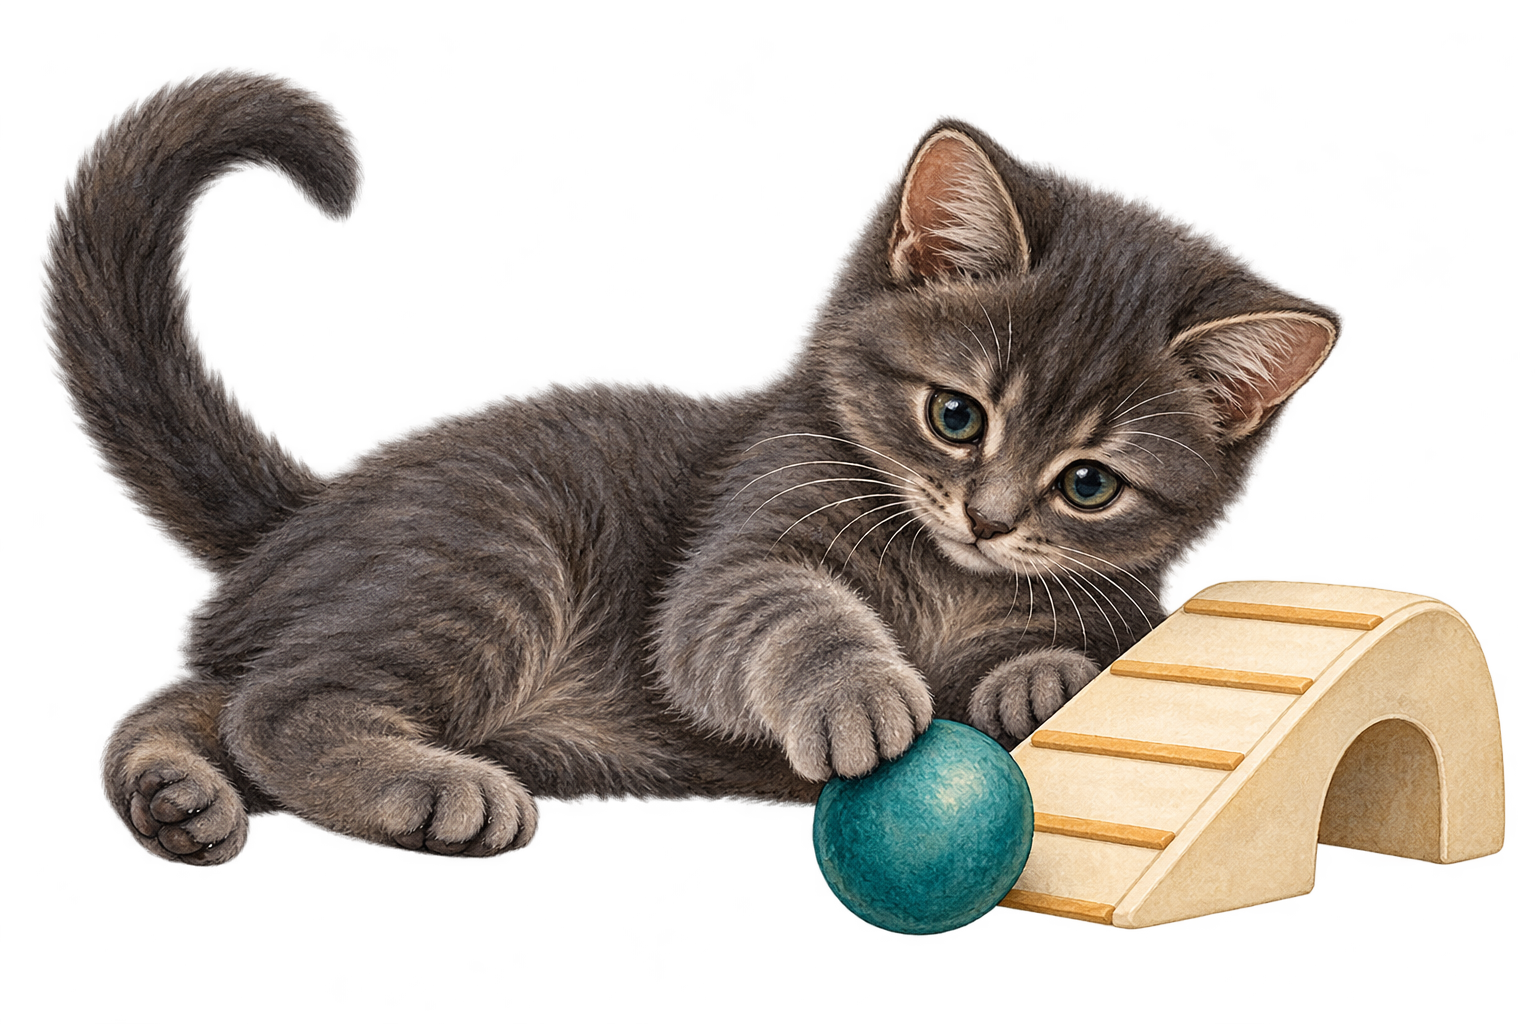
\includegraphics[width=54mm,height=58mm,keepaspectratio]{images/unique/art-209.png}
\end{wrapfigure}
\textit{Доказательство.} Складываем равенства \(A_t=D_{t-1}-D_t+rD_{t-1}\). Разности соседних остатков сокращаются; на полном сроке остаётся \(D_0-D_n=P\), на части срока — \(D_{l-1}-D_m\).\hfill\(\blacksquare\)
\par\WFclear\end{minipage}\end{lrbox}%
\ifdim\dimexpr\ht\CatFlowBox+\dp\CatFlowBox\relax<58mm\dp\CatFlowBox=\dimexpr58mm-\ht\CatFlowBox\relax\fi%
\noindent\usebox{\CatFlowBox}\par\addvspace{2pt}

\begin{example}[Два разных темпа уменьшения]\label{ex:review-ege-exam-models-2}
Кредит \(240000\) рублей берут на четыре периода под \(10\%\). После платежей остатки должны составить \(180000,120000,90000,0\). В первых двух периодах основной долг уменьшается на \(60000\), затем на \(30000\), затем на \(90000\). Платежи равны
\[
84000,\quad78000,\quad42000,\quad99000.
\]
Их сумма \(303000=240000+0{,}1(240000+180000+120000+90000)\). За последние два периода платят \(141000\), а не половину всей суммы: по формуле части срока это \(120000+0{,}1(120000+90000)\).
\end{example}
Если остаток долга несколько периодов сохраняется на уровне \(D\), каждый соответствующий платёж равен только начисленным процентам \(rD\). После такого участка последующие платежи рассчитываются по оставшемуся долгу, а не по сумме уже выплаченных процентов.

\section{Оптимальный выпуск и условие окупаемости}
\begin{example}[Сначала выбрать выпуск, затем цену]\label{ex:review-ege-exam-models-3}
Строительство стоит \(54\) млн рублей. При выпуске \(q\ge0\) тыс. изделий годовые затраты \(\frac12q^2+q+2\) млн, цена \(p\) тыс. рублей за изделие. Годовая прибыль
\[
\Pi(q)=pq-\frac12q^2-q-2
=-\frac12(q-(p-1))^2+\frac12(p-1)^2-2.
\]
При \(p\le1\) максимум на \(q\ge0\) достигается при \(q=0\) и равен \(-2\), окупаемости нет. При \(p>1\) оптимальный выпуск \(q=p-1\). Для окупаемости не более чем за три года нужна максимальная годовая прибыль хотя бы \(18\), поэтому \(\frac12(p-1)^2-2\ge18\). Получаем \(p\ge1+2\sqrt{10}\). Наименьшая действительная цена \(1+2\sqrt{10}\), оптимальный выпуск \(2\sqrt{10}\). В модели выпуск непрерывен; при требовании целого количества нужно отдельно проверить соседние целые выпуски.
\end{example}

\begin{example}[Неравенство с весами из бюджетной модели]\label{ex:review-ege-exam-models-4}
Два производства выпускают за неделю \(x,y\ge0\) единиц; затраты \(100x^2+300y^2\) не превышают \(120000\) рублей. По Коши--Буняковскому
\[
(x+y)^2=
\left((10x)\frac1{10}+(10\sqrt3y)\frac1{10\sqrt3}\right)^2
\le(100x^2+300y^2)\left(\frac1{100}+\frac1{300}\right)
\le1600.
\]
Следовательно, \(x+y\le40\). Равенство требует \(100x=300y\), то есть \(x=3y\), и полного использования бюджета. Значения \(x=30,y=10\) удовлетворяют обоим условиям. Поэтому \(40\) — достижимый максимум, а не только верхняя оценка.
\end{example}
\Needspace{7\baselineskip}\section*{Задачи}
\begingroup\setlength{\parskip}{1pt}
\noindent\begin{minipage}[t]{\linewidth}\textbf{17.1.} Поезд идёт \(2{,}5\) часа со скоростью \(84\) км/ч. Найди путь.\par\end{minipage}\par
\noindent\begin{minipage}[t]{\linewidth}\textbf{17.2.} Два пешехода идут навстречу из пунктов на расстоянии \(27\) км со скоростями \(4\) и \(5\) км/ч. Когда встретятся?\par\end{minipage}\par
\noindent\begin{minipage}[t]{\linewidth}\textbf{17.3.} Велосипедист со скоростью \(18\) км/ч догоняет другого, едущего \(12\) км/ч с отрывом \(9\) км. Через сколько часов догонит?\par\end{minipage}\par
\noindent\begin{minipage}[t]{\linewidth}\textbf{17.4.} Половину пути автомобиль едет \(40\), половину --- \(60\) км/ч. Найди среднюю скорость.\par\end{minipage}\par
\noindent\begin{minipage}[t]{\linewidth}\textbf{17.5.} Полчаса автомобиль едет \(40\), затем полчаса --- \(60\) км/ч. Найди среднюю скорость.\par\end{minipage}\par
\par\addvspace{2pt}\begin{lrbox}{\CatFlowBox}\begin{minipage}[t]{\linewidth}
\setlength{\parskip}{2pt}\setlength{\columnsep}{4.5mm}\setlength{\intextsep}{0pt}
\begin{wrapfigure}[11]{r}{54mm}

\includegraphics[width=54mm,height=58mm,keepaspectratio]{images/unique/art-210.png}
\end{wrapfigure}
\textbf{17.6.} Катер проходит \(24\) км по течению за \(2\) часа, против --- за \(3\) часа. Найди собственную скорость и скорость течения.\par

\textbf{17.7.} Два станка отдельно выполняют заказ за \(12\) и \(18\) часов. Сколько времени нужно вместе при постоянной независимой работе?\par

\textbf{17.8.} Вместе мастера делают работу за \(4\) часа, первый один --- за \(6\). За сколько часов справится второй?\par

\textbf{17.9.} Труба наполняет бак за \(5\) часов, слив опустошает за \(10\). Когда полный бак получится из пустого при совместной работе?\par
\par\WFclear\end{minipage}\end{lrbox}%
\ifdim\dimexpr\ht\CatFlowBox+\dp\CatFlowBox\relax<58mm\dp\CatFlowBox=\dimexpr58mm-\ht\CatFlowBox\relax\fi%
\noindent\usebox{\CatFlowBox}\par\addvspace{2pt}

\noindent\begin{minipage}[t]{\linewidth}\textbf{17.10.} Рабочий сделал половину заказа за \(3\) часа. Сколько времени займёт оставшаяся часть при производительности на \(50\%\) больше?\par\end{minipage}\par
\noindent\begin{minipage}[t]{\linewidth}\textbf{17.11.} Смешали \(200\) г \(10\%\)-го и \(300\) г \(20\%\)-го растворов. Найди концентрацию.\par\end{minipage}\par
\noindent\begin{minipage}[t]{\linewidth}\textbf{17.12.} К \(400\) г \(15\%\)-го раствора добавили \(200\) г воды. Найди концентрацию.\par\end{minipage}\par
\noindent\begin{minipage}[t]{\linewidth}\textbf{17.13.} Из \(500\) г \(12\%\)-го раствора выпарили \(100\) г чистой воды. Найди концентрацию остатка.\par\end{minipage}\par
\noindent\begin{minipage}[t]{\linewidth}\textbf{17.14.} Из \(10\) л однородного \(20\%\)-го по объёму раствора отлили \(2\) л и долили \(2\) л воды. Предположи аддитивность объёмов. Найди новую долю.\par\end{minipage}\par
\noindent\begin{minipage}[t]{\linewidth}\textbf{17.15.} К \(200\) г \(10\%\)-го раствора добавляют чистую соль до \(25\%\). Сколько соли нужно?\par\end{minipage}\par
\noindent\begin{minipage}[t]{\linewidth}\textbf{17.16.} Сумма \(50000\) рублей растёт по простым процентам \(8\%\) за год три года. Найди итог.\par\end{minipage}\par
\noindent\begin{minipage}[t]{\linewidth}\textbf{17.17.} Та же сумма растёт три года по сложным процентам \(8\%\) за год. Найди итог без промежуточного округления.\par\end{minipage}\par
\noindent\begin{minipage}[t]{\linewidth}\textbf{17.18.} Цена \(800\) рублей сначала выросла на \(25\%\), затем снизилась на \(10\%\). Найди итог.\par\end{minipage}\par
\noindent\begin{minipage}[t]{\linewidth}\textbf{17.19.} После снижения на \(20\%\) товар стоит \(960\) рублей. Какова исходная цена?\par\end{minipage}\par
\noindent\begin{minipage}[t]{\linewidth}\textbf{17.20.} Кредит \(100000\) рублей: в конце года начисляют \(10\%\), затем платят \(60000\). Найди остаток.\par\end{minipage}\par
\noindent\begin{minipage}[t]{\linewidth}\textbf{17.21.} Для кредита из предыдущей задачи какой второй платёж через ещё год полностью погасит долг?\par\end{minipage}\par
\noindent\begin{minipage}[t]{\linewidth}\textbf{17.22.} Кредит \(100000\) рублей погашают за два периода по \(10\%\) с равными основными частями долга. Найди платежи.\par\end{minipage}\par
\noindent\begin{minipage}[t]{\linewidth}\textbf{17.23.} Кредит \(210000\) рублей под \(10\%\) за период погашают двумя равными платежами в конце периодов. Найди платёж и переплату.\par\end{minipage}\par
\noindent\begin{minipage}[t]{\linewidth}\textbf{17.24.}\starmark{} Долг \(P\) гасят тремя равными основными частями; ставка \(5\%\) за период. Полная выплата \(66000\). Найди \(P\).\par\end{minipage}\par
\noindent\begin{minipage}[t]{\linewidth}\textbf{17.25.} Прямоугольник имеет периметр \(28\). Найди наибольшую площадь.\par\end{minipage}\par
\noindent\begin{minipage}[t]{\linewidth}\textbf{17.26.} Выручка от продажи \(q\) изделий равна \(q(100-q)\), \(q\) --- целое, \(0\le q\le100\). При каком \(q\) она наибольшая?\par\end{minipage}\par
\noindent\begin{minipage}[t]{\linewidth}\textbf{17.27.}\starmark{} При цене \(p\) спрос \(q=51-p\). Допустимы целые \(p\) от \(1\) до \(50\). Максимизируй выручку \(pq\).\par\end{minipage}\par
\noindent\begin{minipage}[t]{\linewidth}\textbf{17.28.}\starmark{} Докажи, что средняя скорость на двух равных участках при \(u,v>0\) равна \(\dfrac{2uv}{u+v}\) и не превосходит \(\dfrac{u+v}2\).\par\end{minipage}\par
\noindent\begin{minipage}[t]{\linewidth}\textbf{17.29.}\starmark{} Докажи, что концентрация смеси двух растворов положительных масс лежит между их концентрациями.\par\end{minipage}\par
\par\addvspace{2pt}\begin{lrbox}{\CatFlowBox}\begin{minipage}[t]{\linewidth}
\setlength{\parskip}{2pt}\setlength{\columnsep}{4.5mm}\setlength{\intextsep}{0pt}
\begin{wrapfigure}[11]{l}{54mm}

\includegraphics[width=54mm,height=58mm,keepaspectratio]{images/unique/art-290.png}
\end{wrapfigure}
\textbf{17.30.}\starmark{} Вклад \(P\) пополняют суммой \(B\) в конце каждого из \(n\) периодов, после начисления ставки \(r>0\). Выведи сумму после последнего пополнения.\par

\textbf{17.31.}\starmark{} Смешивают неизвестные массы \(20\%\)-го и \(60\%\)-го растворов. После добавления \(12\) кг воды концентрация \(30\%\); если вместо воды добавить \(12\) кг \(50\%\)-го раствора, концентрация \(40\%\). Найди обе исходные массы.\par

\textbf{17.32.}\starmark{} Кредит \(300000\) рублей возвращают за три периода. После платежей долг должен равняться \(240000,120000,0\). В начале каждого периода начисляется одна ставка \(r\), затем вносится платёж. Общая выплата \(399000\). Найди ставку и все три платежа.\par

\textbf{17.33.}\starmark{} Кредит \(120000\) рублей погашают за четыре месяца равными основными частями долга. Перед каждым платежом начисляют \(2\%\) на остаток. Сколько составит сумма платежей за последние два месяца?\par
\par\WFclear\end{minipage}\end{lrbox}%
\ifdim\dimexpr\ht\CatFlowBox+\dp\CatFlowBox\relax<58mm\dp\CatFlowBox=\dimexpr58mm-\ht\CatFlowBox\relax\fi%
\noindent\usebox{\CatFlowBox}\par\addvspace{2pt}

\noindent\begin{minipage}[t]{\linewidth}\textbf{17.34.}\starmark{} Кредит \(P\) взят на четыре года под \(10\%\) с начислением перед платежом. Первые два года основной долг не уменьшается; в последние два года кредит полностью гасят двумя равными платежами. Общая выплата \(284000\) рублей. Найди \(P\) и платежи.\par\end{minipage}\par
\noindent\begin{minipage}[t]{\linewidth}\textbf{17.35.}\starmark{} Создание предприятия стоит \(48\) млн рублей. Годовые затраты при выпуске \(q\ge0\) тыс. изделий равны \(\dfrac12q^2+2q+2\) млн рублей. Цена изделия \(p\) тыс. рублей; выпуск ежегодно выбирают для максимальной прибыли. При какой наименьшей действительной цене строительство окупится не более чем за три года?\par\end{minipage}\par
\noindent\begin{minipage}[t]{\linewidth}\textbf{17.36.}\starmark{} В непрерывной модели два цеха выпускают \(x,y\ge0\) единиц продукции при затратах \(100x^2+400y^2\) рублей. Бюджет \(50000\). Каков наибольший общий выпуск? Найди распределение выпуска и проверь бюджет.\par\end{minipage}\par
\endgroup
